\chapter{Phase and Frequency Stability Measures}
\label{chap:time_stability}

\section{Introduction}

Timekeeping requires a periodic event that can be counted and a time reference point.  In order to synchronize two clocks, it is necessary to match the frequency of the periodic event and transfer the reference point. Figuring out the reference point requires calculating an approximate delay due to propagation, which can be achieved by transmitting a time point and then waiting to receive confirmation from the other system. The White Rabbit Project achieves synchronization by using Synchronous Ethernet for syntonization, and the IEEE $1588$ Precision Time Protocol \cite{Serrano2013} to determine the initial time point. 

However, no frequency source is perfect; there are initialization errors, manufacturing flaws, and environmental influences. Environmental sources for oscillator instability include pressure, temperature, and magnetic fields \cite{blair1974time}. 
%There are excellent references on the history of clocks and oscillator errors \cite{Leeson2016} \cite{Allan1997}.
This thesis investigates the instabilities caused by optical impairments from the fiber medium and amplifiers. Environmental effects or issues inherent to the oscillator source have been treated in other studies \cite{blair1974time,Sliwczynski2010,Sliwczynski2015}.

A frequency source can be represented as 
%
\begin{equation}
	\label{eq:freqsignal}
	u_c(t) = [U_0 + \epsilon(t)] \sin[\omega_0t + \phi(t)]
\end{equation}
%
where $U_0$ is the amplitude and $\epsilon(t)$ is amplitude fluctuation. The quantity $\omega_0=2\pi f_0$ is the nominal angular frequency, and $\phi(t)$ is the phase fluctuation. The amplitude fluctuation must be much less than the nominal amplitude, $|\epsilon(t)| \ll |U_0|$; similarly, the frequency fluctuation, given by the time derivative of the phase, $\dot{\phi} \equiv d\phi/dt$, must be much less than the nominal angular frequency, $|\dot{\phi}| \ll |\omega_0|$. Otherwise, the frequency signal is too heavily distorted to be useful.

A clock can only give a meaningful time with respect to another clock; for instance, the wall clock should match in some way with the position of the sun (which we can consider to be a natural clock). If a clock is fast or slow, it is only in reference to another clock used as a standard. Consider the phases of two different clocks,
%
\begin{equation}
\omega_1(t) = 2\pi f_1t + \phi_1(t), \qquad \omega_2(t) = 2\pi f_2t + \phi_2(t),
\end{equation}
%
then comparing the times when the two are in phase, $\omega_1(t_{n1}) = \omega_2(t_{n2})$. The time difference between the two is
%
\begin{equation}
t_{n1} - t_{n2} = \left[\frac{f_2 - f_1}{f_1f_2}\right] - \left[\frac{\phi_1(t_{n1})}{2\pi f_1} + \frac{\phi_2(t_{n2})}{2\pi f_2}\right].
\end{equation}
%
The terms in the right bracket represent a phase drift, so if we suppose that any long-term drift in the system is compensated, then we have only a short-term phase instability which we assume has zero mean. Averaging over several of these matched phase terms, we have
%
\begin{equation}
\Delta t = \langle t_{n1} - t_{n2} \rangle = \frac{f_2 - f_1}{f_1f_2} = \frac{\Delta f}{f}T,
\end{equation}
%
where $\Delta t$ is the time deviation, $T$ is a total time, and $\Delta f/f$ is the fractional frequency. For example, an atomic clock based on the cesium standard has fractional frequency of $3 \times 10^{-15}$, this means it has a time deviation of $\pm 1$ sec in $10$ million years \cite{CsFracFreq}.

Most of the literature on time and frequency control uses the fractional frequency, denoted $y(t)$, and the phase time, $x(t)$, \cite{Kartaschoff1978, Allan1974, Riley1994}
%
\begin{equation}
\label{eq:phasefreqquantities}
y(t) = \frac{\omega(t) - \omega_0}{\omega_0} = \frac{\dot{\phi}(t)}{\omega_0}, \;\;\;\;\; x(t) = \int_0^t y(\tau)d\tau = \frac{\phi(t)}{\omega_0}.
\end{equation}
%
where $\omega(t) = \omega_0 + \dot{\phi}(t)$ is the instantaneous frequency. However, it is useful for our theoretical study to work mainly with $\phi$ and $\dot{\phi}$. Using $\phi$ and $\dot{\phi}$ emphasizes the phase and frequency deviations of the signal and is more convenient in theoretical work, whereas the fractional frequency and phase time are better suited for physical measurements. Note also that $x$ and $\phi$ are measured instantaneously because they are based on the phase of the clock, and as detailed in the previous paragraph, measuring $y$ requires a time average
%
\begin{equation} \label{eq:avgy}
\bar{y}_k = \frac{1}{\tau}\int_{t_k}^{t_k+\tau} y(t)dt,
\end{equation}
%
where the index $k$ refers to some specific time $t_k$.

Since the errors have a random component, the use of statistical measures like the power spectral density (PSD) is necessary. In general, the variations in time and frequency measurements cannot be described as a stationary process and defining a variance in the usual sense is not possible \cite{Allan1974, blair1974time}. This difficulty led to the invention of the Allan variance \cite{Allan1974, blair1974time}. Structure functions are another approach to characterising phase and frequency variations \cite{Lindsey1976}. In this chapter, we will describe these different approaches and then show the relationships among them.

\section{Power Spectral Density} \label{sec:psd}

The PSD of the phase noise can be obtained by feeding the output of a phase demodulator into a spectrum analyser, and, similarly, the PSD of the frequency noise can be obtained by feeding the output of a frequency demodulator into a spectrum analyzer \cite{blair1974time}.

For any of the quantities $w=x$, $y$, $\phi$, or $\dot{\phi}$ the autocorrelation is defined as
%
\begin{equation}
\label{eq:autocorr}
R_w(\tau) = \langle w(t)w(t+\tau) \rangle = \lim\limits_{T\to\infty}\frac{1}{T}\int_{0}^{T} w(t)w(t+\tau)dt,
\end{equation}
%
and the corresponding PSDs are the Fourier transforms of the autocorrelations
%
\begin{align}
S_w(\omega) &= 2\int_0^\infty R_w(\tau)\cos(\omega\tau)d\tau \\
R_w(\tau) &= \frac{1}{\pi}\int_0^\infty S_w(\omega)\cos(\omega\tau)d\omega
\end{align}
%
Evaluating $R_w(\tau)$ at $\tau = 0$ gives us the second moment of $w$, 
%
\begin{equation*}
R_w(0) = \langle [w(t)]^2 \rangle = \int_0^\infty S_w(\omega) d\omega
\end{equation*}
%
which we refer to as the signal power. If we compare the PSD of two different sources, then the one with the lower signal power will typically have less error.

The PSDs for each of our quantities are related. We find
%
\begin{subequations}
\begin{align}
S_{\dot{\phi}}(\omega) &= \omega^2 S_\phi(\omega), \\
S_y(\omega) &= \frac{\omega^2}{\omega_0^2}S_\phi(\omega), \\
S_x(\omega) &= \frac{1}{\omega_0^2}S_\phi(\omega).
\end{align}
\end{subequations}
%
The oscillator noise can typically be decomposed into a power series $S_\phi(\omega) = \sum_{k=0}^{4} h_k\omega^{-k}$ \cite{Riley1994}. The term proportional to $\omega^0$ is referred to as white phase noise, the term proportional to $\omega^{-1}$ is referred to as flicker phase noise, and the term proportional to $\omega^{-2}$ is referred to as random walk phase noise. Since $S_{\dot{\phi}}(\omega) = \omega^2 S_\phi(\omega)$, the powers in the series increase by $2$. The term proportional to $\omega^{-3}$ is referred to as flicker frequency noise, and the term proportional to $\omega^{-4}$ is referred to as random walk frequency noise \cite{Kartaschoff1978, LohWhite, LohFlicker, NISTFreqStandards}. Figure~\ref{fig:PSD} shows the different noise regions for the PSDs of the fractional frequency $y$ and the phase noise $\phi$.
%
\begin{figure}[htp]
	\centering
	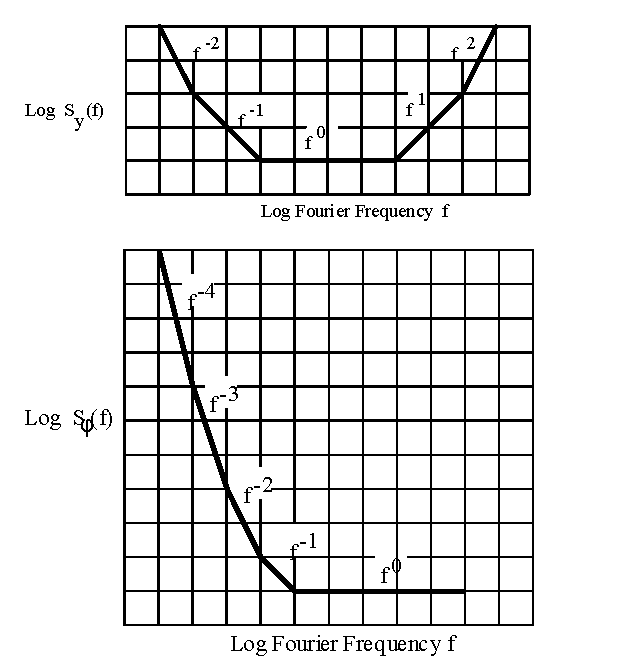
\includegraphics[scale=0.9]{img/PSD.pdf}
	\caption{Power Spectral Density model from \cite{PSDFigure}} \label{fig:PSD}
\end{figure}

\section{Allan Variance} \label{sec:avar}

The distribution of the frequency errors is difficult to determine because it is typically nonstationary.  The sample variance from finitely many measurements may not converge to the true variance of the process as the number of samples goes to infinity. The Allan variance is the mean of sample variances calculated over an interval. The definition is based on the fractional frequency $y$ and phase time $x$; however, we will express it in terms of the phase $\phi$. We use the averaged quantity $\bar{y}_k$ defined in Eq.~\ref{eq:avgy}.

The $N$-sample mean is defined as
%
\begin{equation}
\mu = \frac{1}{N} \sum_{k=1}^{N} \bar{y}_k.
\end{equation}
%
The $N$-sample mean can then be used to compute the $N$-sample variance,
%
\begin{equation}
\sigma_S^2(N) = \frac{1}{N-1} \sum_{k=1}^{N} \left(\bar{y}_k - \mu\right)^2 = \frac{1}{N-1} \sum_{k=1}^{N} \left(\bar{y}_k - \frac{1}{N} \sum_{i=1}^{N} \bar{y}_i\right)^2.
\end{equation}
%
The Allan variance $\sigma^2_A$ \cite{Allan1974} is the mean of the sample variances over all time,
%
\begin{equation}
\sigma_A^2(N,\tau) = \langle \sigma_S^2(N) \rangle = \bigg\langle \frac{1}{N-1} \sum_{k=1}^{N} \left(\bar{y}_k - \frac{1}{N} \sum_{i=1}^{N} \bar{y}_i\right)^2 \bigg\rangle.
\end{equation}
%
In general, the Allan variance utilises $N$ samples, where $N$ can have any integer value greater than $1$, but typically the $N=2$ two-sample Allan variance is used, for which
%
\begin{equation} \label{eq:2sallan}
\sigma_A^2(2, \tau) = \frac{1}{2}\langle [\bar{y}_{k+1} - \bar{y}_{k}]^2 \rangle.
\end{equation}
%
It is not possible to average over all time; so, one computes the Allan variance from a total set of $M$ samples. One then obtains
%
\begin{equation}
\sigma_A^2(\tau,M) = \frac{1}{2(M-1)}\sum_{k=1}^{M-1} \left(\bar{y}_{k+1} - \bar{y}_{k}\right)^2
\end{equation}
%
where it is understood that $N=2$ in the definition of $\sigma_A^2(\tau,M)$.
The averaged fractional frequency is related to the phase by the relationship $\bar{y}_k = [\phi(t_k+\tau) - \phi(t_k)]/(\omega_0\tau)$. Hence, the Allan variance may be written in terms of the phase as
% 
\begin{equation} \label{eq:phiallan}
\sigma_A^2(\tau) = \frac{1}{2}\bigg\langle \left[\frac{\phi(t_k+2\tau) - \phi(t_k+\tau)}{\omega_0\tau} - \frac{\phi(t_k+\tau) - \phi(t_k)}{\omega_0\tau}\right]^2 \bigg\rangle.
\end{equation}
Since the fractions in the average are similar to the discrete derivative, we see that the Allan variance defined in this way refers to the short-term frequency stability, i.e. $\dot{\phi}/\omega_0$.

The Allan deviation is usually plotted in the literature and is the square root of the Allan variance. Allan deviation is usually depicted as the symbol $\sigma_y(\tau)$, $\sigma_A(\tau)$, or ADEV.

\section{Structure Functions} \label{sec:structure}

The definitions of the structure functions are based on studies that Kolmogorov performed on turbulence \cite{Lindsey1976}. The oscillator phase $\phi(t)$ can be written as the statistical process
%
\begin{equation} \label{eq:phaseprocess}
\phi(t) = \omega_0t + \sum_{k=2}^{N} \frac{\Omega_{k-1}}{k!}t^k + \psi(t) + \phi_0
\end{equation}
%
where $\psi(t)$ is the short-term phase fluctuation, which can be considered a stationary process, and $\phi_0$ is a constant. The remaining terms take into account the long-term phase drift. This long-term drift is the source of nonstationarity. The structure functions can be used to remove the long-term drift from $\phi(t)$. 

The first difference equation
%
\begin{equation}
\Delta\phi(\tau) \equiv \Delta\phi(t;\tau) = \phi(t+\tau) - \phi(t)
\end{equation}
%
is the total phase accumulated over the interval $\tau$. The $N$-th difference equation is defined recursively, using
%
\begin{equation}
\Delta^N\phi(\tau) = \Delta^{N-1}\left[\Delta\phi(\tau)\right].
\end{equation}
%
Whenever the process $\phi(t)$ is a stationary process, the mean of the $N$-th difference equation is $0$. The $N$-th order structure function is then the second moment of the $N$-th difference equation,
\begin{equation}
D_\phi^{(N)}(\tau) = \langle [\Delta^N\phi(\tau)]^2 \rangle.
\end{equation}
%
Since the first difference equation is the total phase accumulation, the function $[D_\phi^{(1)}(\tau)]^{1/2}$ equals the mean phase accumulation. Dividing the first difference equation by the time difference $\tau$ is equivalent to discrete differentiation in time, so that $[\phi(t+\tau) - \phi(t)]/\tau$ is the discrete frequency accumulation over $\tau$, and the standard deviation of this term is the mean frequency accumulation \cite{Lindsey1976}.

The random process need not be stationary in order for the difference equation to be stationary. For example, if the process is the sum of an $n$-th order polynomial in time with an additive stationary process, then the $M$-th difference equation eliminates all the polynomial terms whenever $M > n$, and we are left with the $M$-th difference of the stationary process. 

For a stationary process, there is a further simplification for the first-order structure function. Expanding this structure function, we find
%
\begin{equation}
\label{eq:structureexpansion}
\langle [\phi(t+\tau) - \phi(t)]^2 \rangle = \langle \phi(t+\tau)\phi(t+\tau) + \phi(t)\phi(t) - 2\phi(t+\tau)\phi(t) \rangle.
\end{equation}
%
The first two terms on the right-hand-side of the equation are the variance of the process $\phi$ because it is stationary, and we obtain
%
\begin{equation}
\label{eq:structuretoautocorr}
\langle [\phi(t+\tau) - \phi(t)]^2 \rangle = 2R_\phi(0) - 2R_\phi(\tau)
\end{equation}
%
where $R_\phi(\tau)$ is the autocorrelation defined in Eq.~\ref{eq:autocorr}. The structure functions can be computed to higher accuracy using less data than the correlation function \cite{Schulz-DuBois1981}. This advantage is particularly noticeable for flicker noise, whose power spectral density is proportional to $\omega^{-1}$ and is commonly present in oscillators.

\section{Converting between different measures} \label{sec:convert}
%
The power spectral density (PSD) is the most fundamental measure of frequency stability. However, sampling the time data points over a sufficiently long time to accurately obtain the PSD at low frequencies can be difficult. In particular, there may not be enough frequency resolution to obtain the low frequency deviations proportional to $\omega^{-1}$ \cite{LohFlicker}. When the PSD is available, the structure functions and the Allan variance can be obtained from it. The reverse is not generally true, although it is sometimes possible through the use of Mellin transformations \cite{Kartaschoff1978, Lindsey1976}.

\subsubsection*{Allan variance to the second-order structure function:}
%
We now show that the Allan variance is proportional to the second-order structure function. Using the definition of Allan variance in Eq.~\ref{eq:phiallan}, we obtain
%
\begin{align} \label{eq:avtosf}
\nonumber \sigma_A^2(2, \tau) &= \frac{1}{2}\bigg\langle \left[\frac{\phi(t_k+2\tau) - \phi(t_k+\tau)}{\omega_0\tau} - \frac{\phi(t_k+\tau) - \phi(t_k)}{\omega_0\tau}\right]^2 \bigg\rangle \\
&= \frac{1}{2\omega_0^2\tau^2} \langle\left[ \phi(t_k+2\tau) - 2\phi(t_k+\tau) + \phi(t_k) \right]^2\rangle.
\end{align}
%
The $t_k$ are arbitrary when averaging over all time; so, the ensemble average is equal to the structure function $D_\phi^{(2)}(\tau)$ divided by $2\omega_0^2$.

\subsubsection*{PSD to structure functions:}
%
The relation between the PSD and the structure function depends on the long-term frequency drift of the oscillator and whether the $M$-th difference equation is stationary \cite{Lindsey1976}. Suppose that the drift is compensated or $M > N$, where $N$ is the highest-order polynomial term for the drift, then we find
%
\begin{equation}
	D_\phi^{(M)}(\tau) = 2^{2M}\int_{-\infty}^{\infty} \sin^{2M}\left( \frac{\omega\tau}{2}\right) S_\phi(\omega) d\omega.
\end{equation}

\subsubsection*{PSD to Allan variance:}
%
Since we demonstrated that the Allan variance is proportional to a structure function in Eq.~\ref{eq:avtosf}, we combine the results from the last two sections, and we obtain
%
\begin{equation}
\sigma_A^2(2,\tau) = \frac{2^2}{\omega_0^2\tau^2} \int_{-\infty}^{\infty} \sin^4\left( \frac{\omega\tau}{2} \right) S_\phi(\omega) d\omega.
\end{equation}

\section{Chapter remarks} \label{sec:2conc}
%
We will be using the structure functions, specifically $D^{(1)}_\phi(\tau)$, as our preferred measure of stability. The reason for this choice is that it requires fewer samples to compute the flicker noise, and it is simple to implement and interpret. We will also use the Allan deviation to characterize the stability because it is a common measure of frequency stability in the oscillator community, and we can obtain it from the structure function $D_\phi^{(2)}(\tau)$. The phase noise PSD is preferred for experimental measurements.

